\chapter{Wave Nature of Matter}
\label{p:wsl:wnm12}

\section{Introduction}
% Note to Editors: This chapter should perhaps be moved later in the book, as some information which is supposed to be known only comes after this chapter!}

In chapters \ref{p:em:emr12} and \ref{p:mm:op12} the so-called wave-particle duality of light is described. This duality states that light displays properties of both waves and of particles, depending on the experiment performed. For example, interference and diffraction of light are properties of its  wave nature, while the photoelectric effect is a property of its particle nature. In fact we call a particle of light a photon.

Hopefully you have realised that nature loves symmetry. So, if light which was originally believed to be a wave also has a particle nature, then perhaps particles, also display a wave nature. In other words matter which we originally thought of as particles may also display a wave-particle duality.
\chapterstartvideo{VPpiy}
\section{de Broglie Wavelength}
%\begin{syllabus}
%\item The learner must be able to derive the formula for calculating the de Broglie wavelength ($\lambda = \frac{h}{mv}$).
%\item The learner must be able to show that a wavelength calculated for something like a moving cricket ball is so small as to be meaningless but that for a fast-moving electron, the wavelength is such as to expect it to undergo diffraction in the right circumstances.
%\item The learner must be able to calculate the de Broglie wavelength for electrons of varying speeds.
%\item The learner must be able to relate the de Broglie wavelength of the electron to wavelengths within the electromagnetic spectrum. i.e. they are much smaller than that of visible light
%\item Learners should already be able to:
%\begin{itemize}
%\item Describe structure of an atom.
%\item Apply the concept of momentum.
%\item Describe the electromagnetic spectrum.
%\item Describe the dual nature of electromagnetic radiation.
%\item Describe that light is transmitted as tiny particles known as photons.
%\end{itemize}
%\end{syllabus}

Einstein showed that for a photon, its momentum, $p$, is equal to its energy, $E$ divided by the speed of light, $c$:
$$p=\frac{E}{c}.$$
The energy of the photon can also be expressed in terms of the wavelength of the light, $\lambda$:
$$E=\frac{hc}{\lambda},$$
where $h$ is Planck's constant. Combining these two equations we find that the the momentum of the photon is related to its wavelength
$$p=\frac{hc}{c\lambda}=\frac{h}{\lambda},$$
or equivalently
$$\lambda=\frac{h}{p}.$$

In 1923, Louis de Broglie proposed that this equation not only holds for photons, but also holds for  particles of matter. This is known as the de Broglie hypothesis.
 
\Definition{De Broglie Hypothesis}{A particle of mass $m$ moving with velocity $v$  has a wavelength $\lambda$ related to is momentum $p=mv$ by \begin{equation}
\lambda=\frac{h}{p}=\frac{h}{mv}\end{equation}
This wavelength, $\lambda$, is known as the de Broglie wavelength of the particle (where $h$ is Planck's constant).
 }

Since the value of Planck's constant is incredibly small $h = 6.63\times10^{-34}~\mathrm{J\cdot s}$, the wavelike nature of everyday objects is not really observable. 

\begin{IFact}
{The de Broglie hypothesis was proposed by French physicist Louis de Broglie (15 August 1892 -- 19 March 1987) in 1923 in his PhD thesis. He was awarded the Nobel Prize for Physics in 1929 for this work, which made him the first person to receive a Nobel Prize on a PhD thesis.}
\end{IFact}

\begin{wex}{de Broglie Wavelength of a Cricket Ball}{A cricket ball has a mass of $0,150\ekg$ and is bowled towards a bowler at $40\ems$. Calculate the de Broglie wavelength of the cricket ball?}
{\westep{Determine what is required and how to approach the problem}
We are required to calculate the de Broglie wavelength of a cricket ball given its mass and speed. We can do this by using:
$$\lambda=\frac{h}{mv}$$

\westep{Determine what is given}
We are given:
\begin{itemize}
\item The mass of the cricket ball $m=0,150\ekg$
\item The velocity of the cricket ball $v=40\ems$
\end{itemize}
and we know:
\begin{itemize}
\item Planck's constant $h=6,63\times 10^{-34}~\mathrm{J\cdot s}$
\end{itemize}

\westep{Calculate the de Broglie wavelength}
\begin{eqnarray*}
\lambda&=&\frac{h}{mv}\\
&=&\frac{6,63 \times 10^{-34}\;\mathrm{J\cdot s}}{(0,150\ekg)(40~\ems)}\\
&=& 1,11 \times 10^{-34}\emm
\end{eqnarray*}
}
\end{wex}
This wavelength is considerably smaller than the diameter of a proton which is approximately $10^{-15}~\emm$. Hence the wave-like properties of this cricket ball are too small to be  observed.

\begin{wex}{The de Broglie wavelength of an electron}
{Calculate the de Broglie wavelength of an electron moving at 40~\ms.}
{
\westep{Determine what is required and how to approach the problem}
We are required to calculate the de Broglie wavelength of an electron given its speed. We can do this by using:
$$\lambda=\frac{h}{mv}$$

\westep{Determine what is given}
We are given:
\begin{itemize}
\item The velocity of the electron {$v=40\ems$}
\end{itemize}
and we know:
\begin{itemize}
\item The mass of the electron {$m_{e}=9,11 \times 10^{-31}\ekg$}
\item Planck's constant {$h=6,63 \times 10^{-34}~\mathrm{J\cdot s}$}
\end{itemize}

\westep{Calculate the de Broglie wavelength}
\begin{eqnarray*}
\lambda&=&\frac{h}{mv}\\
&=&\frac{6,63\times10^{-34}~\mathrm{J\cdot s}}{(9,11 \times 10^{-31}\ekg)(40~\ems)}\\
& = & 1,82 \times 10^{-5}\emm\\
&=&0,0182\;\mathrm{mm}
\end{eqnarray*}
}
\end{wex}


Although the electron and cricket ball in the two previous examples are travelling at the same velocity the de Broglie wavelength of the electron is much larger than that of the cricket ball. This is because the wavelength is inversely proportional to the mass of the particle.

\begin{wex}{The de Broglie wavelength of an electron}
{Calculate the de Broglie wavelength of a electron moving at $3 \times 10^{5}\ems$. ($\frac{1}{1000}$ of the speed of light.)}

{\westep{Determine what is required and how to approach the problem}
We are required to calculate the de Broglie wavelength of an electron given its speed. We can do this by using:
$$\lambda=\frac{h}{mv}$$

\westep{Determine what is given}
We are given:
\begin{itemize}
\item The velocity of the electron {$v=3 \times 10^{5}\ems$}
\end{itemize}
and we know:
\begin{itemize}
\item The mass of the electron {$m=9,11 \times 10^{-31}\ekg$}
\item Planck's constant {$h=6,63\times10^{-34}~\mathrm{J\cdot s}$}
\end{itemize}

\westep{Calculate the de Broglie wavelength}
\begin{eqnarray*}
\lambda&=&\frac{h}{mv}\\
&=&\frac{6,63\times10^{-34}~\mathrm{J\cdot s}}{(9,11 \times 10^{-31}\ekg)(3 \times 10^{5}\ems)}\\
& = & 2,43 \times 10^{-9}\emm
\end{eqnarray*}
This is the size of an atom. For this reason, electrons moving at high velocities can be used to ``probe" the structure of atoms. This is discussed in more detail at the end of this chapter.  Figure \ref{rel-wave-leng} compares the wavelengths of fast moving electrons to the wavelengths of visible light.}
\end{wex}

Since the de Broglie wavelength of a particle is inversely proportional to its velocity, the wavelength decreases as the velocity increases. This is confirmed in the last two examples with the electrons. 
De Broglie's hypothesis was confirmed by Davisson and Germer in 1927 when they observed a beam of electrons being diffracted off a nickel surface. The diffraction means that the moving electrons have a wave nature. They were also able to determine the wavelength of the electrons from the diffraction. To measure a wavelength one needs two or more diffracting centres such as pinholes, slits or atoms. For diffraction to occur the centres must be separated by a distance about the same size as the wavelength. Theoretically, all objects, not just sub-atomic particles, exhibit wave properties according to the de Broglie hypothesis.

\begin{figure}[htbp]
\begin{center}
\begin{pspicture}(-1.2,-1.2)(8.2,1)
%\psgrid[gridcolor=gray]
\psline{<->}(-0.5,0)(8,0)
\psline{->}(0.02,0.5)(0.02,0.2)
\uput[u](0.02,0.5){fast electrons}
\uput[d](0.02,0){$\approx$ 2~nm}

\psline{->}(4,0.5)(4,0.2)
\psline{->}(7,0.5)(7,0.2)
\uput[u](5.5,0.2){visible light}
\uput[d](4,0){$\approx$ 700~nm}
\uput[d](7,0){$\approx$ 400~nm}
\rput(4.25,-1){wavelength (nm)}
\end{pspicture}
\caption{The wavelengths of the fast electrons are much smaller than that of visible light.}
\label{rel-wave-leng}
\end{center}
\end{figure}

\section{The Electron Microscope}
%\begin{syllabus}
%\item The learner must be able to compare, by means of a simple diagram, the principle of operation of an electron microscope with an optical microscope in terms of the specimen, focusing and image formation.
%\item[Advanced] The learner must be able to explain that electron microscopes, both transmission (TEM) and scanning (SEM), produce images based on the wave properties of electrons, just as light microscopes produce images based on the wave properties of light.
%\item[Advanced] The learner must be able to state that extremely small de Broglie wavelengths of high-speed electrons permit imaging with a high resolution and magnification, whereas the magnification of a light microscope is limited by the wavelength of light.
%\item[Advanced] The learner must be able to compare the internal operating mechanisms of the light microscope with the transmission electron microscope.
%\begin{itemize}
%\item source: Light Microscope (visible light transmitted through specimen, focussing mechanism: optical lenses, imaging: the eye
%\item source: Transmission Electron Microscope (TEM) (invisible beam of electrons transmitted through specimen, focussing mechanism: magnetic field of solenoid (acts like a converging lens for electrons), imaging: fluorescent screen or photographic plate
%\end{itemize}
%\item[Advanced] The learner must be able to discuss the differences between the operation of the transmission electron microscope (TEM) and the scanning electron microscope (SEM).
%\end{syllabus}

We have seen that under certain circumstances particles behave like waves. This idea is used in the electron microscope which is a type of microscope that uses electrons to create an image of the target. It has much higher magnification or resolving power than a normal light microscope, up to two million times, allowing it to see smaller objects and details.


Let's first review how a regular optical microscope works.  A beam of light is shone through a thin target and the image is then magnified and focused using objective and ocular lenses. The amount of light  which passes through the target depends on the densities of the target since the less dense regions allow more light to pass through than the denser regions. This means that the beam of light which is partially transmitted through the target carries information about the inner structure of the target. 

The original form of the electron microscopy, transmission electron microscopy, works in a similar manner using electrons. In the electron microscope, electrons which are emitted by a cathode are formed into a beam using magnetic lenses. This electron beam is then passed through a very thin target. Again, the regions in the target with higher densities stop the electrons more easily. So, the number of electrons which pass through the different regions of the target depends on their densities. This means that the partially transmitted beam of electrons carries information about the densities of the inner structure of the target. The spatial variation in this information (the "image") is then magnified by a series of magnetic lenses and it is recorded by hitting a fluorescent screen, photographic plate, or light sensitive sensor such as a CCD (charge-coupled device) camera. The image detected by the CCD may be displayed in real time on a monitor or computer. In figure \ref{fig:polio} is an image of the polio virus obtained with a transmission electron microscope.

\begin{figure}[H]
\begin{center}
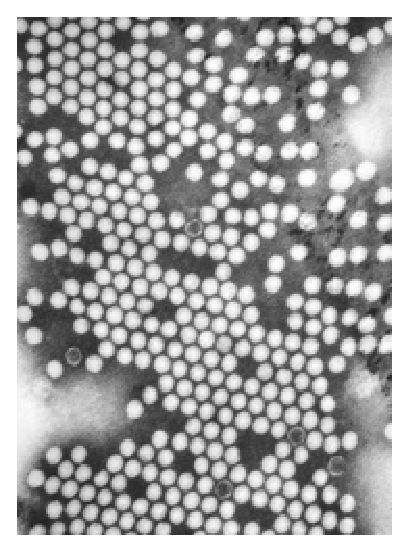
\includegraphics[width=0.25\textwidth]{../../epsimages/mm-Polio.eps}
\caption{The image of the polio virus using a transmission electron microscope.}
\label{fig:polio}
\end{center}
\end{figure}

The structure of an optical and electron microscope are compared in figure \ref{fig:p:wsl:wnm12:lvsem}. While the optical microscope uses light and focuses using lenses, the electron microscope uses electrons and focuses using electromagnets.


\begin{figure}[H]
\begin{center}
\begin{pspicture}(-1.4,-0.6)(8.4,10)
%\psgrid[gridcolor=gray]
\def\lightbulb{\pscircle(0,1){0.5}\psframe(-0.25,0)(0.25,0.5)}
\def\maglens{\psset{yunit=0.75}
\psarc(0,0){0.5}{0}{180}
\psarc(0,0){1}{0}{180}
\psframe(0.5,-0.5)(1,0)
\psframe(-1,-0.5)(-0.5,0)
\psarc(0,-0.5){0.5}{0}{180}
}
\rput(5,0){
\psline{->}(0,9)(0,0.5)
\rput(0,9){\psframe(-0.2,0)(0.2,1)}\uput[r](0.5,9.5){electron source}
\rput(0,7){\maglens}\uput[r](1,8){magnetic lens}
\psframe(-1,5.5)(1,5.7)\uput[r](1,5.6){target}
\rput(0,4){\maglens}\uput[r](1,5){objective lens}
\rput(0,2){\maglens}\uput[r](1,2){projector lens}
\psframe(-1,0)(1,1)\uput[r](1,0.5){screen}
\uput[d](0,0){electron microscope}
}

\rput(0,0){\rput{270}(0,0){\psset{unit=0.5}\eye}
\rput{180}(0,10){\lightbulb}\uput[r](0.5,9.5){light source}
\rput{90}(0,8){\psset{unit=0.7}\lens[lensGlass=true,drawing=false]} \uput[r](1,8){condenser lens}
\psframe(-1,5.5)(1,5.7)\uput[r](1,5.6){target}
\rput{90}(0,5){\psset{unit=0.5}\lens[lensGlass=true,drawing=false]} \uput[r](1,5){objective lens}
\rput{90}(0,2){\psset{unit=0.7}\lens[lensGlass=true,drawing=false]} \uput[r](1,2){eyepiece lens}
\uput[d](0,0){optical microscope}
\psline{->}(0,8.5)(0,1)
}
\end{pspicture}
\caption{Diagram of the basic components of an optical microscope and an electron microscope.}
\label{fig:p:wsl:wnm12:lvsem}
\end{center}
\end{figure}


Electron microscopes are very useful as they are able to magnify objects to a much higher resolution. This is because their de Broglie wavelengths are so much smaller than that of visible light. You hopefully remember that light is diffracted by objects which are separated by a distance of about the same size as the wavelength of the light. This diffraction then prevents you from being able to focus the transmitted light into an image. So the sizes at which diffraction occurs for a beam of electrons is much smaller than those for visible light. This is why you can magnify targets to a much higher order of magnification using electrons rather than visible light.

\begin{table}
\begin{center}
\caption{Comparison of Light and Electron Microscopes}
\begin{tabular}{|c||p{5cm}|p{5cm}|}\hline
& {\bf Light microscope} & {\bf Electron microscope} \\ \hline
Source & Bright lamp or laser & Electron gun \\ \hline
Radiation & U.V. or visible light & Electron beam produced by heating metal surface (e.g. tungsten)\\\hline
Lenses & Curved glass surfaces & Electromagnets\\\hline
Receiver & Eye; photographic emulsion or digital image & Fluorescent screen (for location and focusing image); photographic emulsion or digital image\\\hline
Focus & Axial movement of lenses (up and down)& Adjustment of magnetic field in the electromagnets by changing the current \\\hline
Operating & Atmospheric & High vacuum\\  Pressure & &  \\ \hline
\end{tabular}
\end{center}
\end{table}

\Extension{High-Resolution Transmission Electron Microscope (HRTEM)}{

There are high-resolution TEM (HRTEM) which have been built. In fact the resolution is sufficient to show carbon atoms in diamond separated by only 89 picometres and atoms in silicon at 78 picometres. This is at magnifications of 50 million times. The ability to determine the positions of atoms within materials has made the HRTEM a very useful tool for nano-technologies research. It is also very important for the development of semiconductor devices for electronics and photonics.

Transmission electron microscopes produce two-dimensional images.}

\Extension{Scanning Electron Microscope (SEM)}{
The Scanning Electron Microscope (SEM) produces images by hitting the target with a primary electron beam which then excites the surface of the target. This causes secondary electrons to be emitted from the surface which are then detected.  So the electron beam in the SEM is moved (or scanned) across the sample, while detectors build an image from the secondary electrons.

Generally, the transmission electron microscope's resolution is about an order of magnitude better than the SEM resolution. However, because the SEM image relies on surface processes rather than transmission it is able to image bulk samples (unlike optical microscopes and TEM which require the samples to be thin) and has a much greater depth of view, and so can produce images that are a good representation of the 3D structure of the sample.}

\subsection{Disadvantages of an Electron Microscope}
Electron microscopes are expensive to buy and maintain. They are also very sensitive to vibration and external magnetic fields. This means that special facilities are required to house microscopes aimed at achieving high resolutions. Also the targets have to be viewed in vacuum, as the electrons would scatter off the molecules that make up air. 

\Extension{Scanning Electron Microscope (SEM)}{
Scanning electron microscopes usually image conductive or semi-conductive materials best.  A common preparation technique is to coat the target with a several-nanometre layer of conductive material, such as gold, from a sputtering machine; however this process has the potential to disturb delicate samples.

The targets have to be prepared in many ways to give proper detail. This may result in artifacts purely as a result of the treatment. This gives the problem of distinguishing artifacts from material, particularly in biological samples. Scientists maintain that the results from various preparation techniques have been compared, and as there is no reason that they should all produce similar artifacts, it is therefore reasonable to believe that electron microscopy features correlate with living cells.}

\begin{IFact}
{The first electron microscope prototype was built in 1931 by the German engineers Ernst Ruska and Max Knoll. It was based on the ideas and discoveries of Louis de Broglie. Although it was primitive and was not ideal for practical use, the instrument was still capable of magnifying objects by four hundred times. The first practical electron microscope was built at the University of Toronto in 1938, by Eli Franklin Burton and students Cecil Hall, James Hillier and Albert Prebus.

Although modern electron microscopes can magnify objects up to two million times, they are still based upon Ruska's prototype and his correlation between wavelength and resolution. The electron microscope is an integral part of many laboratories. Researchers use it to examine biological materials (such as microorganisms and cells), a variety of large molecules, medical biopsy samples, metals and crystalline structures, and the characteristics of various surfaces.}
\end{IFact}

\subsection{Uses of Electron Microscopes}
Electron microscopes can be used to study:
\begin{itemize}
\item the topography of an object $-$ how its surface looks.
\item the morphology of particles making up an object  $-$ their shapes and sizes.
\item the composition of an object $-$ the elements and compounds that the object is composed of and the relative amounts of them.
\item the crystallographic information for crystalline samples $-$ how the atoms are arranged in the object.
\end{itemize}

\summary{VPreb}
\begin{itemize}
\item The momentum of a photon can be related to the energy of the photon, $p=\frac{E}{c}$.
\item Combined with $E=\frac{hc}{\lambda}$, a relationship between momentum and wavelength is derived.
\item De Broglie postulated that this relationship holds for all particles and any object has a de Broglie wavelength.
\end{itemize}


\begin{eocexercises}{}
\begin{enumerate}
  \item If the following particles have the same velocity, which has the shortest wavelength: electron, hydrogen atom, lead atom? 
\item A bullet weighing 30 g is fired at a velocity of $500\ems$. What is its wavelength?
\item Calculate the wavelength of an electron which has a kinetic energy of $1.602\times10^{-19}$~J.
\item If the wavelength of an electron is $10^{-9}$~m what is its velocity?
\item Considering how one calculates wavelength using slits, try to explain why we would not be able to physically observe diffraction of the cricket ball in the first worked example.
 \end{enumerate}
% Automatically inserted shortcodes - number to insert 5
\par \practiceinfo
\par \begin{tabular}[h]{cccccc}
% Question 1
(1.)	01it	&
% Question 2
(2.)	01iu	&
% Question 3
(3.)	01iv	&
% Question 4
(4.)	01iw	&
% Question 5
(5.)	01ix	&
\end{tabular}
% Automatically inserted shortcodes - number inserted 5
\end{eocexercises}


% CHILD SECTION END 



% CHILD SECTION START 

